\documentclass[tikz]{standalone}
\usepackage[utf8]{inputenc}
\usetikzlibrary{intersections}

\definecolor{DarkRed}{rgb}{0.7,0.2,0.2}

\begin{document}

% P + (-P) = inf
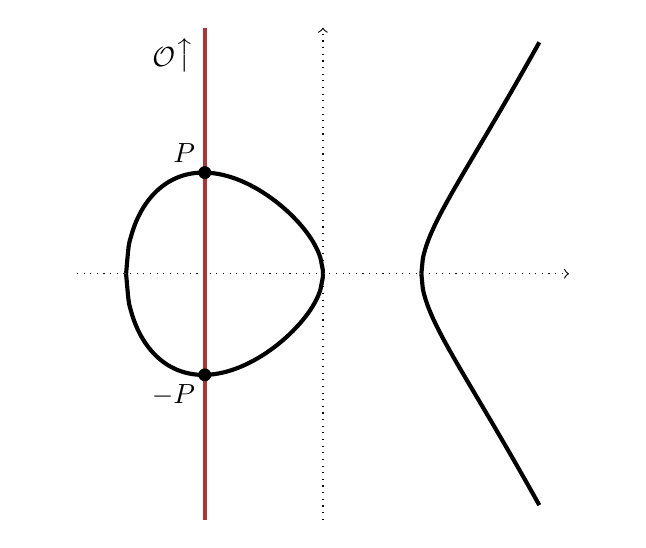
\begin{tikzpicture}[scale=2.5]
\def\ptsize{.03}
\clip (-1.5,-1.25) rectangle (1.5,1.25);
\draw[->,dotted] (-1.25,0) -- (1.25,0);
\draw[->,dotted] (0,-1.25) -- (0,1.25);
\path[domain=-1:0,smooth,samples=80,line width=1.5pt,name path=patatedessus,draw] plot (\x, {sqrt(\x^3 + .5*(\x)^2 - .5*\x)}) -- (0,0);
\path[domain=-1:0,smooth,samples=80,line width=1.5pt,name path=patatedessous,draw] plot (\x, {-sqrt(\x^3 + .5*(\x)^2 - .5*\x)}) -- (0,0);
\path[domain=.5:1.1,smooth,samples=80,line width=1.5pt,name path=branchedessus,draw] plot (\x, {sqrt(\x^3 + .5*(\x)^2 - .5*\x)});
\path[domain=.5:1.1,smooth,samples=80,line width=1.5pt,name path=branchedessous,draw] plot (\x, {-sqrt(\x^3 + .5*(\x)^2 - .5*\x)});
\path[DarkRed,name path=linePQ,line width=1.5pt,draw] (-.6,-1.25) -- (-.6,1.25) node[below left,black] {$\mathcal{O}$\raise1.5pt\hbox{$\big\uparrow$}};
\draw[name intersections={of=patatedessus and linePQ, by=P},fill] (P) circle (\ptsize);
\draw[name intersections={of=patatedessous and linePQ, by=Q},fill] (Q) circle (\ptsize);

\node[above left] at (P) {$P$};
\node[below left] at (Q) {$-P$};
\end{tikzpicture}

\end{document}